\documentclass{slide}
\usepackage{tikz}

\usetikzlibrary{arrows}

\usepackage{tabto}

\usepackage{languages}

% \usepackage{pgfpages}
% \setbeameroption{show notes on second screen}

\title{Distributed Computing II}
\subtitle{CSSE6400}
\author{Brae Webb}
\date{\week{6}}

% \titlegraphic {
%     \tweet%
%     {images/mathiasverraes}%
%     {Mathias Verras}%
%     {mathiasverraes}%
%     {There are only two hard problems in distributed systems:  2. Exactly-once delivery 1. Guaranteed order of messages 2. Exactly-once delivery}%
%     {https://twitter.com/mathiasverraes/status/632260618599403520}%
% }

\begin{document}

\maketitle

\point[Previously in CSSE6400\dots]{
\begin{center}
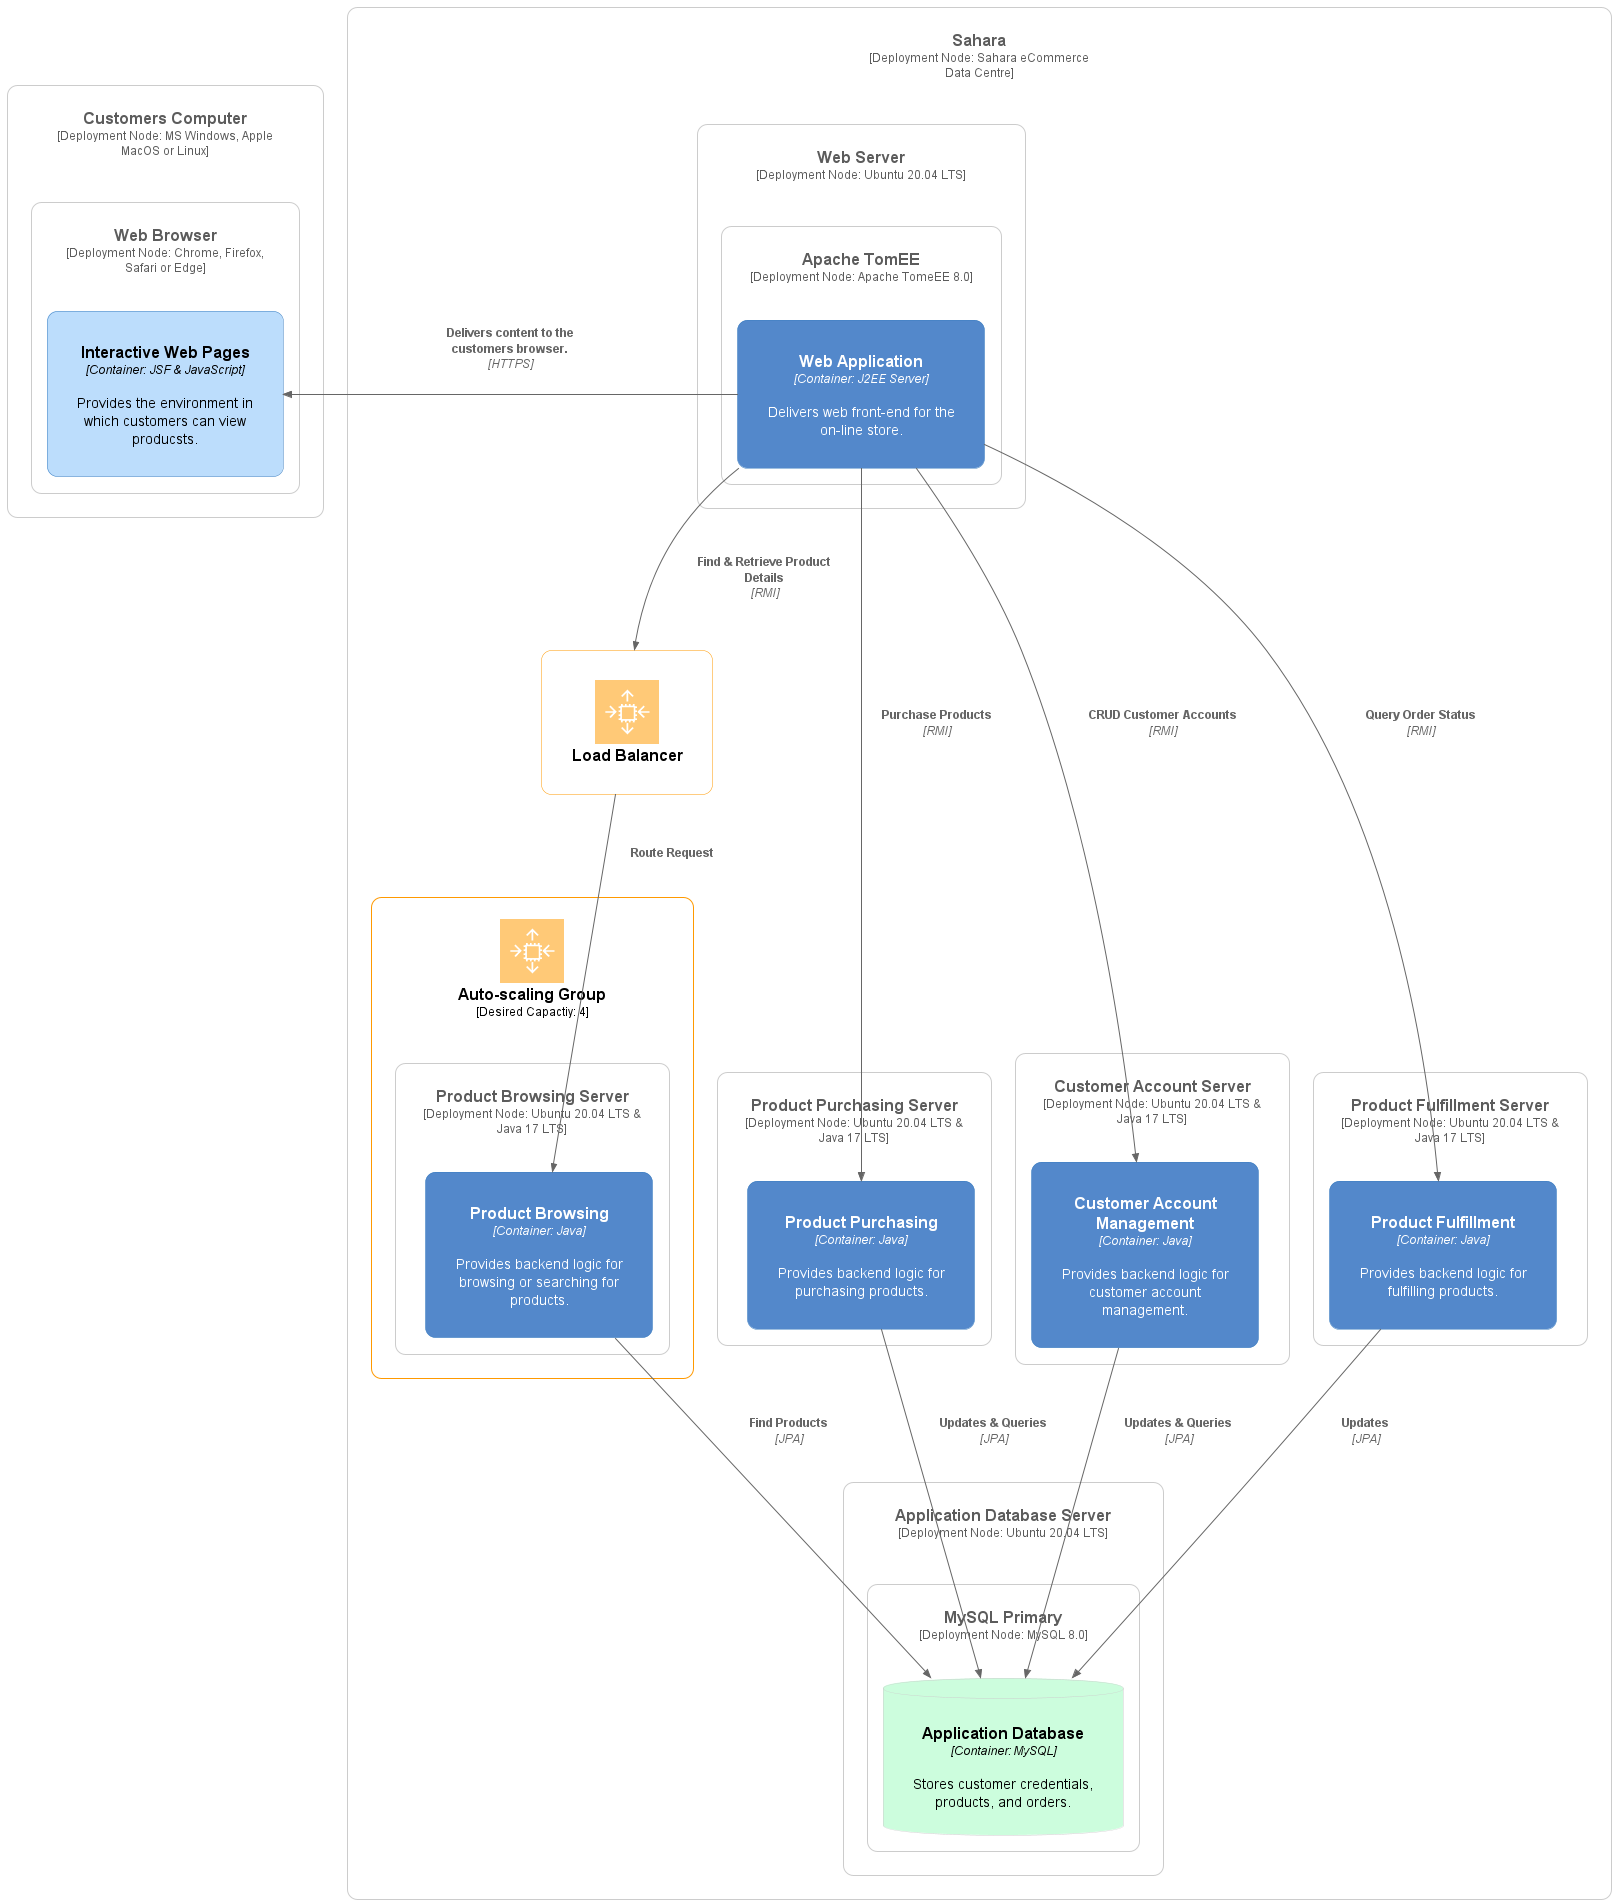
\includegraphics[width=0.8\textheight]{diagrams/SaharaScaled}
\end{center}
}

\note[itemize]{
    \item We scaled a stateless service.
    \item It was stateless as it didn't require persistent data.
    \item This is normally easy to do.
}

\question{What is the \highlight{problem}?}

\note{The database}

\point[Database]{
\begin{center}
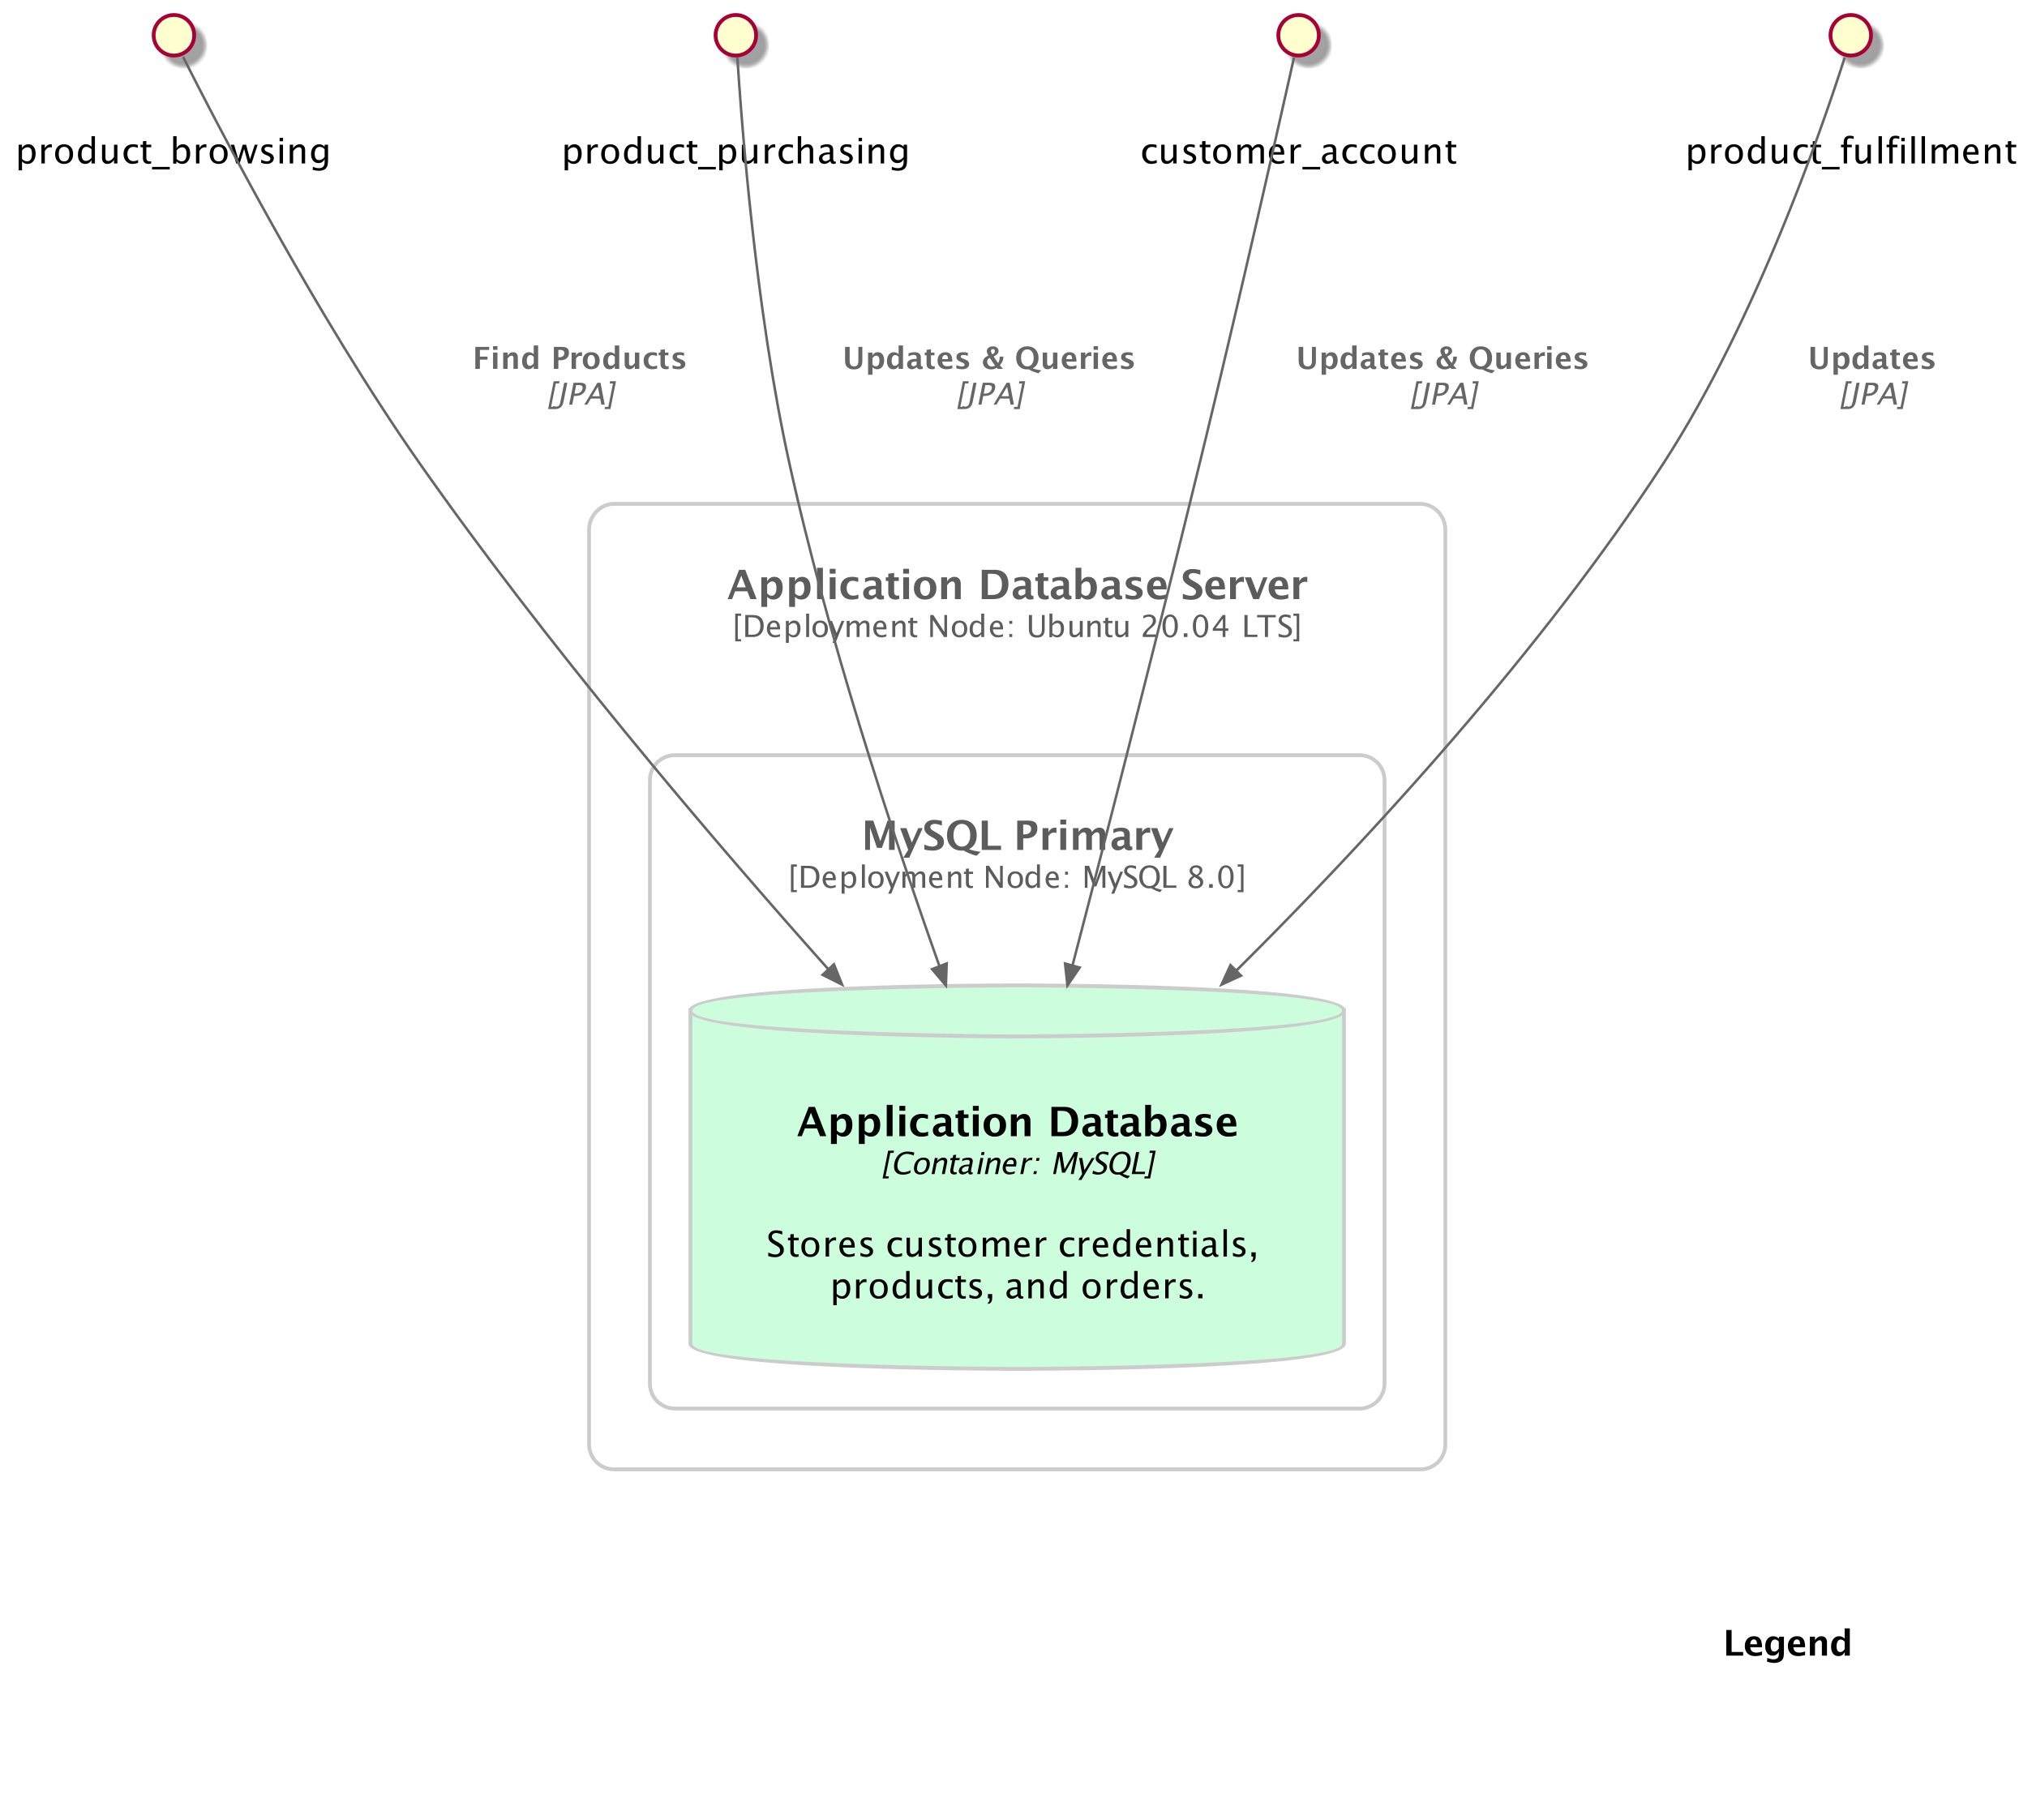
\includegraphics[width=\textheight]{diagrams/FocusDB}
\end{center}
}

\note[itemize]{
    \item The database has state, persistent data.
    \item This is much harder to scale.
}

\point[Disclaimer]{This is \highlight{not} a database course.}

\image{images/infs3200}

\note{This is a database course.}

%%%%%%%%%%%%%%%
% Replication %
%%%%%%%%%%%%%%%
\questionanswer{How do we fix database scaling issues?}{
    \begin{itemize}[<+(1)->]
        \item
        \only<5->{\highlight{Replication}}
        \only<-4>{Replication}
        \item Partitioning
        \item Independent databases
    \end{itemize}
}

\question{What is \highlight{replication}?}

\definition{Replication}{
    Data copied across multiple different machines.
}

\image{diagrams/Replication}

\definition{Replica}{
    Database node which stores a copy of the data.
}


\questionanswer{What are the advantages of \highlight{replication}?}{
    \begin{itemize}[<+(1)->]
        \item Scale out our database to cope with \highlight{load}.
        \item Provide \highlight{fault tolerance} from a single database instance failure.
        \item Locate databases \highlight{closer to end-users}.
    \end{itemize}
}

\note[itemize]{
    \item Scalability
    \item Reliability
    \item Performance
}

\question{How do we replicate our data?}

\note[itemize]{
    \item Easy without updates, just copy it.
    \item Updates, or writes, must propagate changes.
}

\point[First approach]{Leader-follower Replication}

\image{diagrams/LeaderFollower}

\note[itemize]{
    \item Leader-follower is the most common implementation.
    \item Multiple followers, only one leader.
}

\point[Leader-based Replication]{
    \begin{description}[<+->]
        \item[On write] Writes sent to leader, change is propagated via change stream.
        \item[On read] Any replica can be queried. 
    \end{description}
}

\image{diagrams/LeaderFollowerSpread}

\note[itemize]{
    \item Built-in to PostgreSQL, MySQL, MongoDB, RethinkDB, and Espresso.
    \item Can be added to Oracle and SQL Server.
}

\point[Propogating changes]{
    \highlight{Synchronous} vs. \highlight{Asynchronous}
}

\image[height=\textheight]{diagrams/Sync}

\image[height=\textheight]{diagrams/Async}

\image[height=\textheight]{diagrams/SyncVsAsync}

\point[Synchronous propagation]{
\begin{itemize}[<+->]
    \item Writes must propagate to \highlight{all followers} before being successful.
    \item \highlight{Any} replica goes down, \highlight{all} replicas are un-writable.
    \item Writes must \highlight{wait} for propagation to all replicas.
\end{itemize}
}

\point[Asynchronous propagation]{
\begin{itemize}[<+->]
    \item Writes \highlight{don't} have to \highlight{wait} for propagation.
    \item If the leader goes down before propagating, the \highlight{write is lost}.
    \item Replicas can have out-dated or \highlight{stale} data.
\end{itemize}
}

% \todo{There could be content here about handling node failures}

% \point[When things go wrong]{
%     Handling outages
% }

% \point{Follower failure}

% \point{Leader failure}

\definition{Replication Lag}{
    The time taken for replicas to update \highlight{stale} data.
}

\image{diagrams/ReplicationLag}

\note{The time it takes for the change to the name of the product to update across all followers}

\image[height=\textheight]{diagrams/AsyncLag}

\note{The purple part is replication lag}

% \point[The time taken for replicas to update their stale data is]{Replication Lag}

\point[Eventually, all replicas must become consistent]{
    The system is \highlight{eventually consistent}
}

\note[itemize]{
    \item If writes stop for long enough
    \item Eventually is intentionally ambiguous
}

\point[Eventual Consistency]{Problems?}

\begin{frame}
\begin{center}
\tweet%
{images/braewebb}%
{Brae Webb}%
{braewebb}%
{}%
{}%

\only<2->{

\includegraphics[width=0.3\textwidth]{diagrams/ReadYourWrites}
}

\only<3->{
\tweet%
{images/braewebb}%
{Brae Webb}%
{braewebb}%
{}%
{}%
}
\end{center}
\end{frame}

\note[itemize]{
    \item Read user details
    \item Decide I don't like by name
    \item Update name
    \item Read user details
}

\image{diagrams/ReadYourWritesExample}

\definition{Read-your-writes Consistency}{
    Users always see the updates that \highlight{they have made}.
}

\note{Doesn't care what other users see}

\begin{frame}
\begin{center}
\only<1->{
\tweet%
{images/braewebb}%
{Brae Webb}%
{braewebb}%
{My fist post}%
{}%
}

\only<2->{
\tweet%
{images/braewebb}%
{Brae Webb}%
{braewebb}%
{My first post}%
{}%
}

\only<3->{
\tweet%
{images/braewebb}%
{Brae Webb}%
{braewebb}%
{My fist post}%
{}%
}
\end{center}
\end{frame}

\image{diagrams/MonotonicReads}

\definition{Monotonic Reads}{
    Once a user reads an updated value, they don't later see the old value.
}

\note{User doesn't travel back in time}

% \point{Consistent Prefix Reads}
% \todo{Consistent Precix Example}

\point[Summary]{
\begin{itemize}
    \item Leader-follower databases allow \highlight{reads to scale} more effectively.
    \item Asynchronous propagation weakens consistency to \highlight{eventually consistent}.
    \item Leader-follower databases still have a \highlight{leader write bottle-neck}.
\end{itemize}
}

\point[Second approach]{Multi-leader Replication}

\image[height=\textheight]{diagrams/MultiLeader}

\point[Why multi-leader?]{
\begin{itemize}[<+->]
    \item If you have mutliple leaders,
            you can write to any,
            allowing \highlight{writes to scale}.
    \item A leader going down doesn't prevent writes,
            given \highlight{better fault-tolerance}.
\end{itemize}
}

\note[itemize]{
    \item Available via extensions in most databases, often not natively supported.
    \item Best to avoid where possible.
}

% \point[Multi-leader Replication]{Use Cases}

% \note[itemize]{
%     \item Multiple datacenters
%     \item Offline writing
% }

\questionanswer{What might go wrong?}{Write conflicts}

\note{Write conflicts require the conflict to be resolved.}

\image{diagrams/WriteConflict}

\note{-1 Pillows? How do we resolve this?}

\point[Where possible]{Avoid write conflicts}

\image{diagrams/AvoidWriteConflict}

\point[Where impossible]{Convergence}

\point[Convergence Strategies]{
\begin{itemize}[<+->]
    \item Assign each \highlight{write} a unique ID.
    \item Assign each \highlight{leader replica} a unique ID.
    \item Custom resolution logic.
\end{itemize}
}

\image[height=\textheight]{diagrams/ResolveWriteConflict}

\point[Resolving Conflicts]{
\begin{description}
    \item[On Write] When a conflict is first noticed, take proactive resolution action.
    \item[On Read] When a conflict is next read, ask for a resolution.
\end{description} 
}

\note[itemize]{
    \item Bucardo allows a perl script for on write resolution.
    \item CouchDB prompts reads to resolve the conflict.
}

% \point[Cutting Edge]{Automatic Conflict Resolution}

\point[Third Approach]{Leaderless Replication}

\note[itemize]{
    \item Early distributed databases were leaderless.
    \item Resurgance after Amazon created Dynamo.
    \item Dynamo is an internal service and not DynamoDB.
    \item Riak, Cassandra, and Voldemort are leaderless databases.
}

\image{diagrams/Leaderless}

\note{Reads and writes can be written to any node.}

\point[How do they work?]{
    Each read/write is sent to \highlight{multiple} replicas.
}

\image{diagrams/LeaderlessExampleWrite}

\image{diagrams/LeaderlessExampleRead}

\note{At least one of the reads has the updated value}

\point[How are changes propagated?]{
    \begin{itemize}[<+->]
        \item Read Repair
        \item Anti-entropy Process
    \end{itemize}
}

\question{How do we know it's consistent?}

\image{diagrams/LeaderlessExampleBad}

\questionanswer{How do we know it's consistent?}{
    Quorum Reads and Writes
}

\definecolor{eq1}{RGB}{116, 137, 227}
\definecolor{eq2}{RGB}{227, 116, 137}

\point[Quorum Consistency]{
\begin{equation*}
\textcolor{eq1}{w} + \textcolor{eq2}{r} > \textcolor{focus}{n}
\end{equation*}
\Large
\begin{description}
    \item[$\textcolor{focus}{n}$] total replicas
    \item[$\textcolor{eq1}{w}$] amount of replicas to {\color{eq1}\textsl{write}} to
    \item[$\textcolor{eq2}{r}$] amount of replicas to {\color{eq2}\textsl{read}} from
\end{description}
}

\note{The nodes read from must overlap with the nodes written to}

\begin{frame}
\begin{center}
    \begin{tikzpicture}
        \node[anchor=south west,inner sep=0] at (0,0) {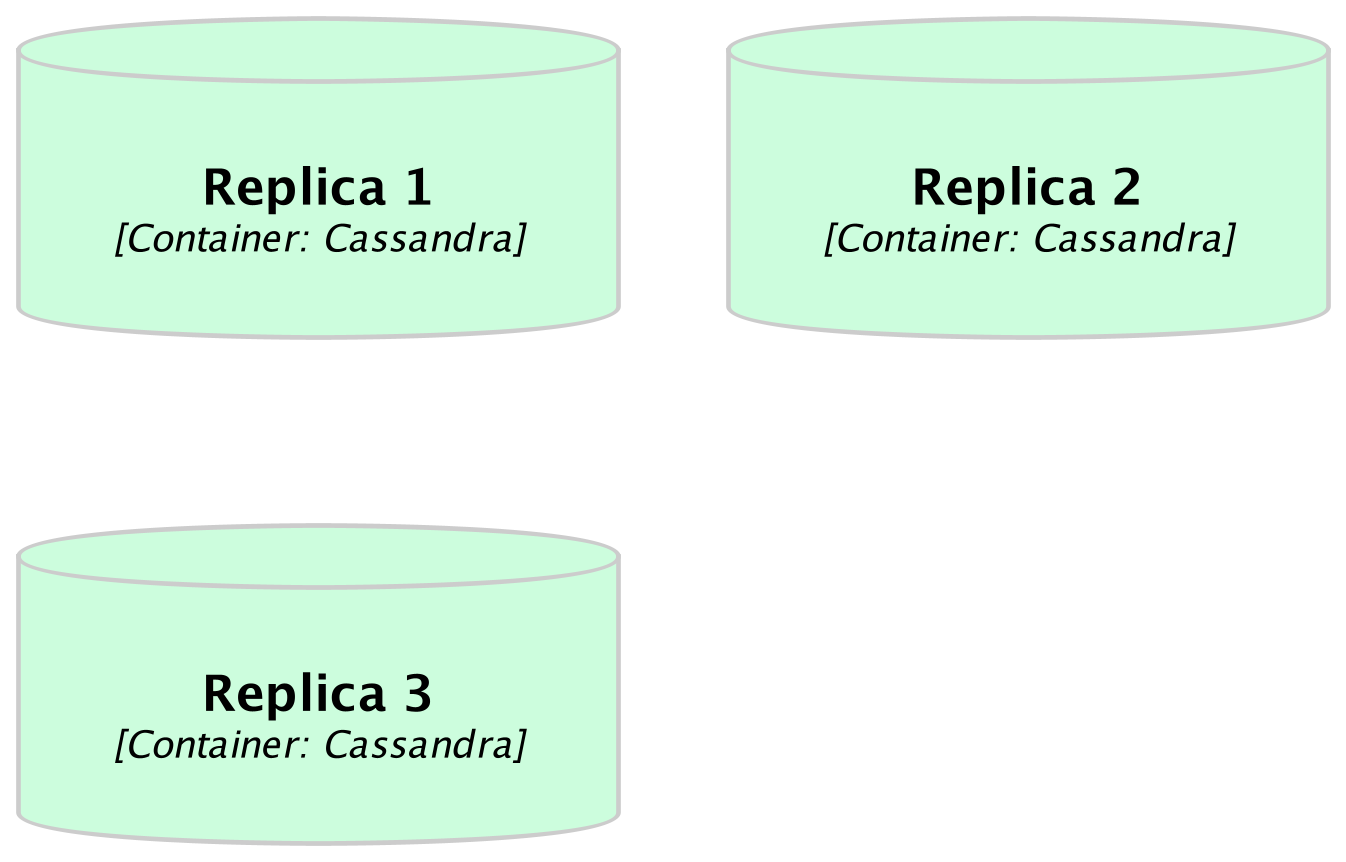
\includegraphics[width=0.8\textwidth]{diagrams/LeaderlessQuorum}};
        \draw[eq1,ultra thick,rounded corners] (0,0) rectangle (5.5,8.2);
        \draw[eq2,ultra thick,rounded corners] (0,4.5) rectangle (11.5,8.2);
        \draw[focus,ultra thick,rounded corners] (-0.1,-0.1) rectangle (11.6,8.3);
        \node at (8.5,3.5) {
            $\textcolor{focus}{n}$ total replicas
        };
        \node at (8.5,2.5) {
            $\textcolor{eq1}{w}$ amount of replicas to {\color{eq1}\textsl{write}} to
        };
        \node at (8.5,1.5) {
            $\textcolor{eq2}{r}$ amount of replicas to {\color{eq2}\textsl{read}} from
        };
    \end{tikzpicture}
\end{center}
\end{frame}

\point[Summary]{
\begin{itemize}[<+->]
    \item \highlight{Replication} copies data to multiple replicas.
    \item \highlight{Leader-based} replication is most common and simpliest.
    \item Replication introduces \highlight{eventual consistency}.
    \item \highlight{Multi-leader} replication scales writes as well as reads but introduces \highlight{write conflicts}.
    \item \highlight{Leaderless} replication is another approach which keeps the problems of multi-leader.
\end{itemize}
}

%%%%%%%%%%%%%%%%
% Partitioning %
%%%%%%%%%%%%%%%%
\questionanswer{How do we fix database scaling issues?}{
    \begin{itemize}
        \item 
        \only<-2>{\highlight{Replication}}
        \only<3->{Replication}
        \item 
        \only<3->{\highlight{Partitioning}}
        \only<-2>{Partitioning}
        \item Independent databases
    \end{itemize}
}

\definition{Partitioning}{
    Split the data of a system onto multiple nodes, these nodes are \highlight{partitions}.
}

\note{Also called shardes, regions, tablets, etc.}

\image{diagrams/Partitioning}

\note[itemize]{
    \item Pioneered in the 1980s
    \item Allow scalability of large data, not just large load.
    \item Partitioning is normally combined with replication.
}

\question{How should we decide which data is stored where?}

\image[height=\textheight]{diagrams/PartitioningExample}

\note{An example partitioning based on primary key, student ID}

\questionanswer{What is the problem with this?}{
    Over time some partitions become inactive,
    while others receive almost all load.
}

\questionanswer{
    How should we decide which data is stored where?
}{
    Maximize spread of requests, avoiding \highlight{skewing}.
}

\questionanswer{Have we seen this before?}{Hashing?}

\note{Hash tables hash entries to maximize the spread between buckets.}

\questionanswer{What is the problem with this?}{
    Range queries are inefficient, i.e. get all students between s4444444 and s4565656
}

\question{How do we route queries?}

\note{Unlike stateless, only one node can process queries.}

\point[Query-insensitive Load Balancer]{
    Randomly route to any node, responsibility of the node to re-route to the correct node.
}

\image{diagrams/PartitioningLB1}

\point[Query-sensitive Load Balancer]{
    A load balancer which understands which queries should be forwarded to which node.
}

\image[height=\textheight]{diagrams/PartitioningLB2}


\point[Client-aware Queries]{
    Place the responsibility on clients to choose the correct node.
}

\image{diagrams/PartitioningLB3}

\point[Summary]{
\begin{itemize}[<+->]
    \item \highlight{Partitioning} splits data across multiple nodes.
    \item A \highlight{consistent method} to chose which node is required.
    \item Partitioning by \highlight{primary key} can create \highlight{skewing}.
    \item Partitioning by \highlight{hash} makes range queries less efficient.
    \item Three approaches to \highlight{routing requests}.
\end{itemize}
}

\point[Disclaimer]{We have ignored the hard parts of replication.}


%%%%%%%%%%%%%%%%%%%%%%%%%%%%%
% Isolation (foreshadowing) %
%%%%%%%%%%%%%%%%%%%%%%%%%%%%%
\questionanswer{How do we fix database scaling issues?}{
    \begin{itemize}
        \item Replication
        \item 
        \only<-2>{\highlight{Partitioning}}
        \only<3->{Partitioning}
        \item 
        \only<3->{\highlight{Independent databases}}
        \only<-2>{Independent databases}
    \end{itemize}
}

% \references{articles,books}

\end{document}